
\section{Experiments}

\begin{table*}[t!]
    \centering
    \small
    \caption{Structure generation results. We report Mean $\pm$ SEM for RMSD and lDDT. RMSD is computed after Kabsch alignment with the true RNA. lDDT is computed on $C_{\alpha}$ atoms.}
    \vspace{0.05in}
    \begin{tabular}{lccc@{\hskip 0.25in}ccc}
        \hline
        \multirow{2}{*}{Method} &
        \multicolumn{2}{c}{\textit{RF2NA Pre-Training Split}} &
        \multicolumn{2}{c}{\textit{Sequence Similarity Split}} \\
        & RMSD & lDDT & RMSD & lDDT \\ \hline
        Conditional MMDiff & $14.82 \pm 1.01$ & $0.34 \pm 0.02$ & $17.42 \pm 0.86$ & $0.38 \pm 0.01$ \\ \hline
        RNAFlow-Base & $12.85 \pm 0.63$ & $0.51 \pm 0.01$ & $14.77 \pm 0.34$ & \textbf{0.57} $\pm$ \textbf{0.01} \\
        RNAFlow-Traj & $13.12 \pm 0.64$ & 0.52 $\pm$ 0.01 & $15.11 \pm 0.33$ & $0.57 \pm 0.00$ \\
        RNAFlow-Base + Rescore & \textbf{10.61} $\pm$ \textbf{1.73} & \textbf{0.53} $\pm$ \textbf{0.03} & \textbf{14.60} $\pm$ \textbf{1.05} & $0.56 \pm 0.02$ \\
        RNAFlow-Traj + Rescore & $15.30 \pm 1.89$ & $0.52 \pm 0.03$ & $15.31 \pm 0.93$ & $0.56 \pm 0.02$ \\
         \hline
        RF2NA [Upper Bound] & $4.67 \pm 1.29$ & $0.76 \pm 0.04$ & $9.83 \pm 1.69$ & $0.79 \pm 0.02$ \\ \hline
    \end{tabular}
    
    \label{tab:1}
\end{table*}



\begin{table*}[h]
    \centering
    \small
    \caption{Sequence generation results. We report Mean $\pm$ SEM for native sequence recovery.}
    \vspace{0.05in}
    \begin{tabular}{lcc@{\hskip 0.25in}cc}
        \hline
        \multirow{2}{*}{Method} &
        \multicolumn{1}{c}{\textit{RF2NA Pre-Training Split}} &
        \multicolumn{1}{c}{\textit{Sequence Similarity Split}} \\
        & Recovery  & Recovery \\ \hline
        Random & $0.25 \pm 0.00$ & $0.25 \pm 0.00$ \\
        LSTM & $0.27 \pm 0.01$ & $0.24 \pm 0.01$ \\
        Conditional MMDiff & $0.24 \pm 0.02$ & $0.22 \pm 0.02$ \\ \hline
        RNAFlow-Base & $0.30 \pm 0.02$ & $0.30 \pm 0.01$ \\ 
        RNAFlow-Traj & $0.31 \pm 0.01$ & $0.28 \pm 0.01$ \\ 
        RNAFlow-Base + Rescoring & $0.33 \pm 0.02$ & \textbf{0.32} $\pm$ \textbf{0.03} \\
        RNAFlow-Traj + Rescoring & \textbf{0.37} $\pm$ \textbf{0.05} & $0.29 \pm 0.02$ \\ \hline
        Inverse Folding [Upper Bound] & $0.46 \pm 0.01$ & $0.35 \pm 0.01$ \\ \hline
    \end{tabular}
    
    \label{tab:2}
\end{table*}

We evaluate RNAFlow in two experimental settings. First, we evaluate RNA sequence and structure prediction error with respect to existing protein-RNA complexes. Dataset construction and results are described in Section \hyperref[sec:exp1]{4.1}. We additionally evaluate the novelty of RNA designs in Section \hyperref[sec:4.2]{4.2}. In Section \hyperref[sec:4.3]{4.3}, we perform an ablation study to determine how modeling choices affect structure and sequence generation.

Second, we evaluate whether RNAFlow can design RNA aptamers for the GRK2 protein, a target of interest for the treatment of chronic heart failure \cite{tesmer2012molecular}. \citet{mayer2008rna} discovered an RNA aptamer that interacts strongly with the GRK2 kinase domain, and \citet{lennarz2015rna} identified $4$ nucleotides that are critical for binding. In Section \hyperref[sec:4.4]{4.4}, we investigate whether RNAFlow can design realistic RNAs for GRK2 binding given this binding site sequence motif.

\subsection{Structure \& Sequence Accuracy}
\label{sec:exp1}

% placement
\begin{figure*}[ht]
    \centering
    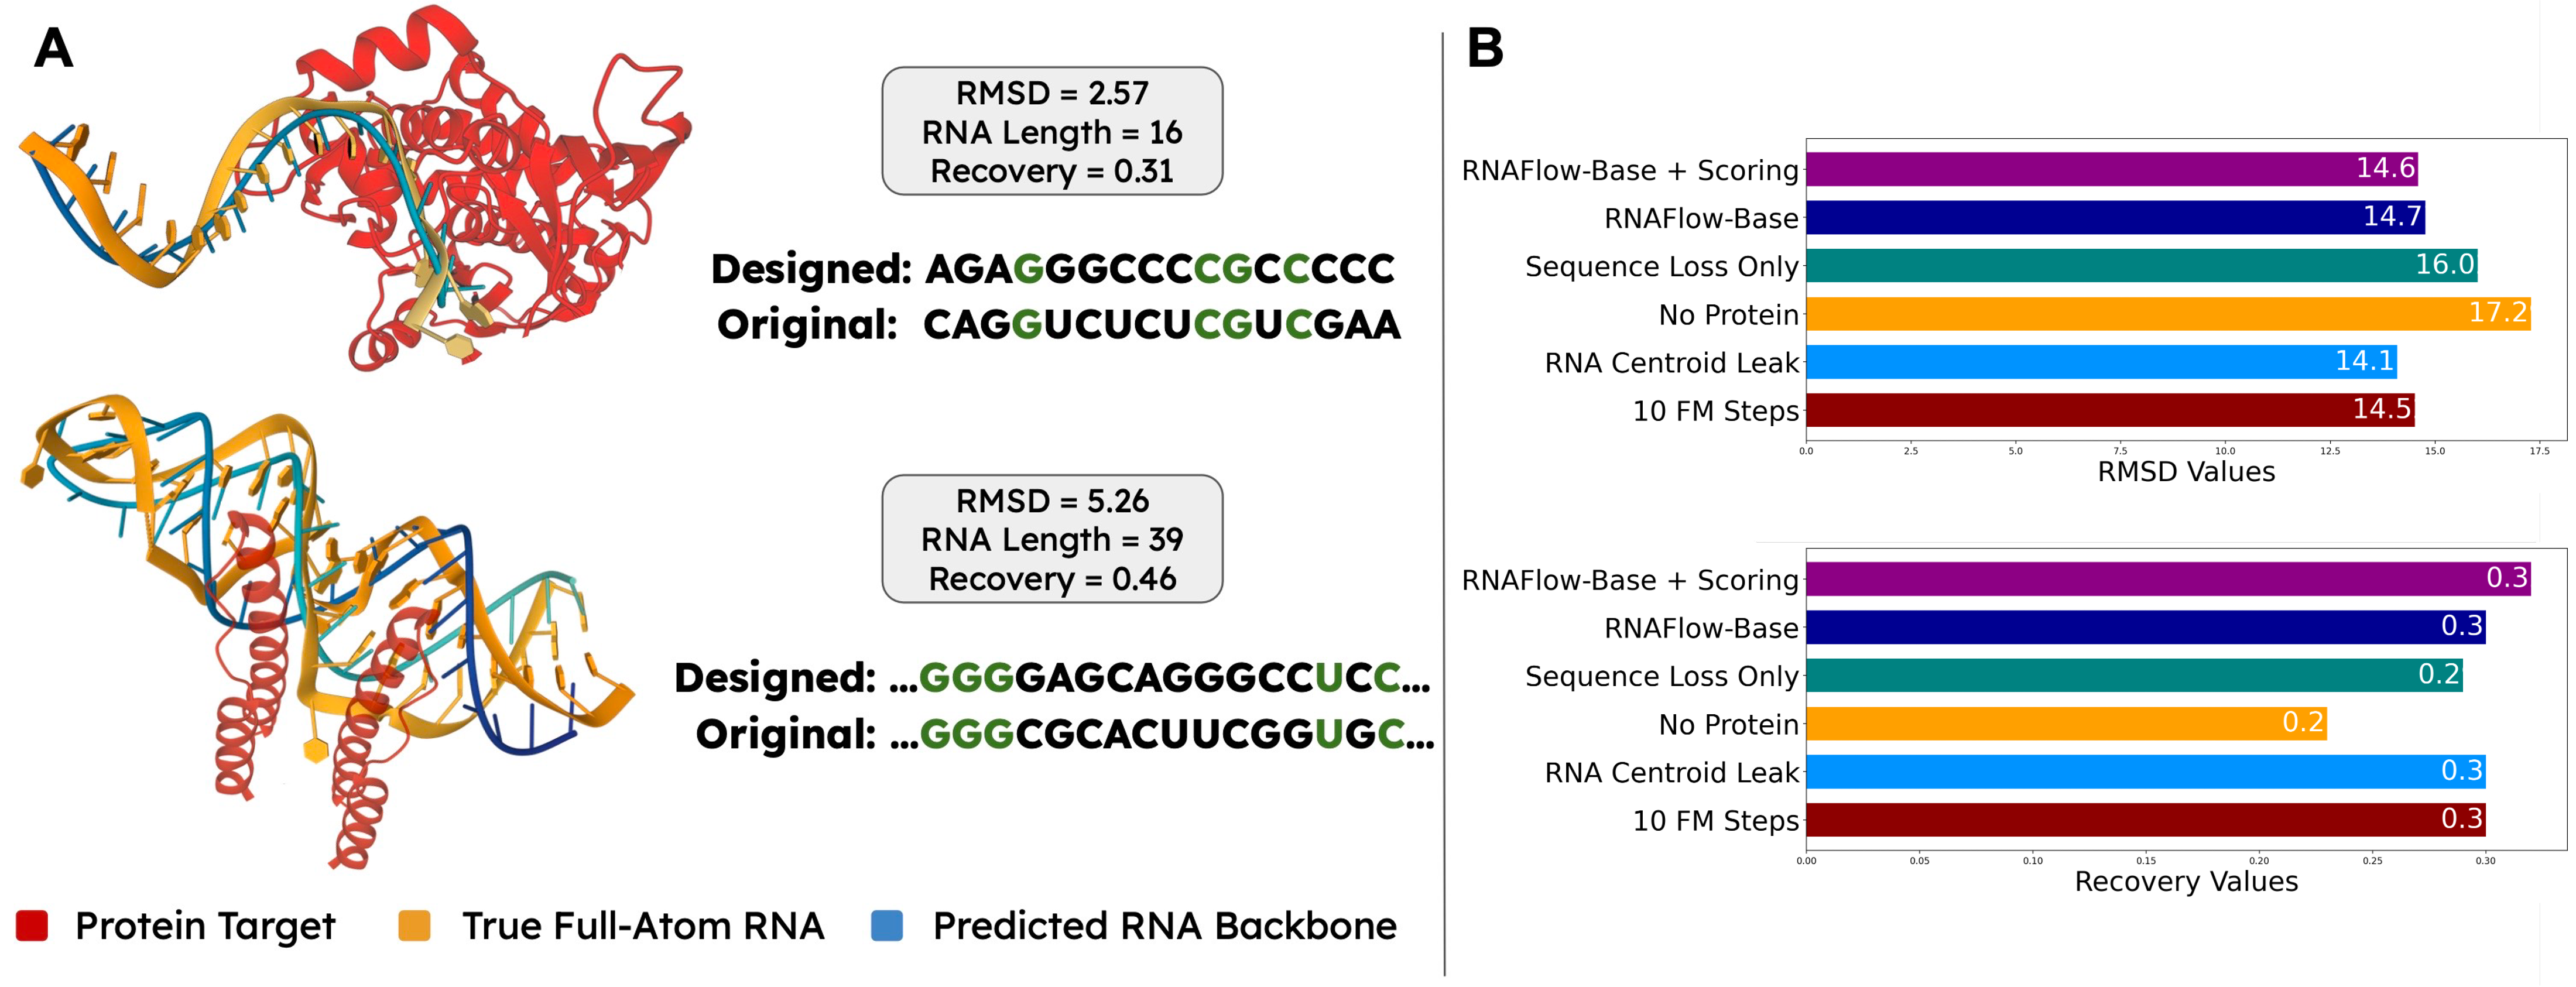
\includegraphics[width=2\columnwidth]{fig3ab_updated.png}
    \caption{(A) Top: Structure and sequence design of RNA for interaction with a viral RNA-dependent RNA polymerase (PDB ID: 4K4X). Bottom: Design of RNA for interaction with HIV-1 Rev protein (PDB ID: 4PMI). (B) Ablation study of RNAFlow components. We report RMSD and sequence recovery on the sequence similarity split.}
    \label{fig:3}
\end{figure*}

As mentioned, we evaluate two variants of our method: \textit{RNAFlow-Base} which is based on Noise-to-Seq and \textit{RNAFlow-Trajectory} which additionally applies Traj-to-Seq. For both methods, we begin by generating $10$ structure-sequence pairs per protein in the test set. From amongst the $10$ designs, we additionally report the performance when $1$ sample is selected by the output rescoring model. All samples are generated with $5$ integration steps.

\textbf{Dataset.} Protein-RNA complexes from the PDBBind dataset (2020 version) were used for training and evaluation \cite{liu2017forging}. Dataset preparation details are described in the Appendix. We perform all experiments on two splits. The first accounts for RF2NA pre-training -- all examples from complexes in the RF2NA validation or test sets were assigned to the test split, and remaining examples were randomly split into training and validation in a $9$:$1$ ratio. To measure how well our model can generalize to dissimilar RNAs, we also evaluate on an RNA sequence similarity split. All RNA chains were clustered using CD-HIT \cite{fu2012cd} where two sequences are in the same cluster if they share $\geq 80\%$ sequence identity, following the clustering protocol of \citet{joshi2023multi}. The clusters were randomly split into train, validation, and test in an $8$:$1$:$1$ ratio. We pre-train Noise-to-Seq on clean protein-RNA complexes before fine-tuning on noised complexes as part of the RNAFlow training loop. Further details are included in the Appendix.

Traj-to-Seq was trained separately on RNASolo \cite{adamczyk2022rnasolo}, a dataset of RNA sequences and structures where many of the sequences are associated with multiple structure conformers. On average, the dataset contains $3$ structures per sequence. Following \citet{joshi2023multi}, we filtered to structures with resolution $\leq 3$ \AA. For the RF2NA split, we curate the Traj-to-Seq training set such that RNAs in our validation and test sets are not used for training. For the sequence similarity split, we remove RNAs that have $\geq 80\%$ similarity with data points in validation/test.  Traj-to-Seq inference was run on the final $3$ structures in the flow matching trajectory which yields optimal performance.

\textbf{Baselines.} For structure generation, we compare our method to two baselines. To our knowledge, the only existing structure generative model for nucleic acids is MMDiff \cite{morehead2023towards}, an $SE(3)$-discrete diffusion model that jointly designs nucleic acid sequences and structures. We sample $10$ RNA designs of the ground-truth RNA's length per protein-RNA complex in our test set, conditioned on the protein backbone structure and sequence. As an upper bound, we compare against RNA structures folded by RF2NA, given the ground-truth protein MSA and RNA sequence. This baseline captures the structure prediction error inherent to our score prediction model.

For sequence generation, we compare our method to four baselines. First, we compare to a random baseline where RNA sequences of specified length are generated by randomly selecting a nucleotide for each position, from a uniform distribution over \{A, C, G, U\}. Next, we compare against sequences designed by MMDiff. Our third baseline is a standard sequence-only model, consisting of an LSTM layer to encode protein sequence $\{p_i\}_{\forall i}$ and an autoregressive LSTM decoder layer to predict RNA sequence $\{\hat r_i\}_{\forall i}$, matching the architecture in \citet{im2019generative}. Finally, we establish an upper bound by comparing against results from our pre-trained inverse folding model, which takes the ground-truth protein-RNA backbone complex as input.

\textbf{Metrics.} For structure generation, we report root mean square deviation (RMSD) between predicted RNA structure and ground-truth structure, computed on all backbone atoms. Before RMSD calculation, the RNA structures are aligned by the Kabsch algorithm. For RNAFlow-Trajectory, we report the average RMSD across structures in the trajectory. We also report lDDT computed on $C_{\alpha}$ atoms. For sequence generation, we report recovery rate which is the percentage of correctly recovered nucleotides in a sampled sequence.

\textbf{Results.} As shown in Table \hyperref[tab:1]{1}, RNAFlow significantly outperforms the baseline on the structure generation task. On the RF2NA and sequence similarity splits respectively, the best RNAFlow model gives a $28\%$ and $16\%$ reduction in RMSD relative to MMDiff. We also observe a $56\%$ and $50\%$ increase in lDDT. Without rescoring, RNAFlow still gives a $13\%$ and $15\%$ reduction in RMSD. However, there is a large gap between the structural accuracy of RNAFlow and RF2NA, given the complexity of the \textit{de novo} design task in comparison to folding. We note that RNAFlow-Trajectory consistently has a higher RMSD than RNAFlow-Base, likely because trajectory structures are taken from earlier points in flow matching inference. We show two examples of generated outputs in Figure \hyperref[fig:3]{3a}, where it is evident that the designed RNA matches the ground truth structure well.

As shown in Table \hyperref[tab:2]{2}, RNAFlow outperforms all baselines on the sequence generation task. On the RF2NA split, the best RNAFlow model gives a $48\%$ improvement over random generation and a $37\%$ improvement over the LSTM baseline. RNAFlow-Trajectory outperforms RNAFlow-Base, suggesting that flow matching trajectories provide useful RNA dynamics information that is not present in a single structure. The output rescoring model improves the mean recovery, indicating that while RNAFlow samples can be variable, we learn to select quality samples. Without rescoring, we see a $15\%$ improvement in recovery relative to the best baseline.

% placement
\begin{figure*}[ht]
    \centering
    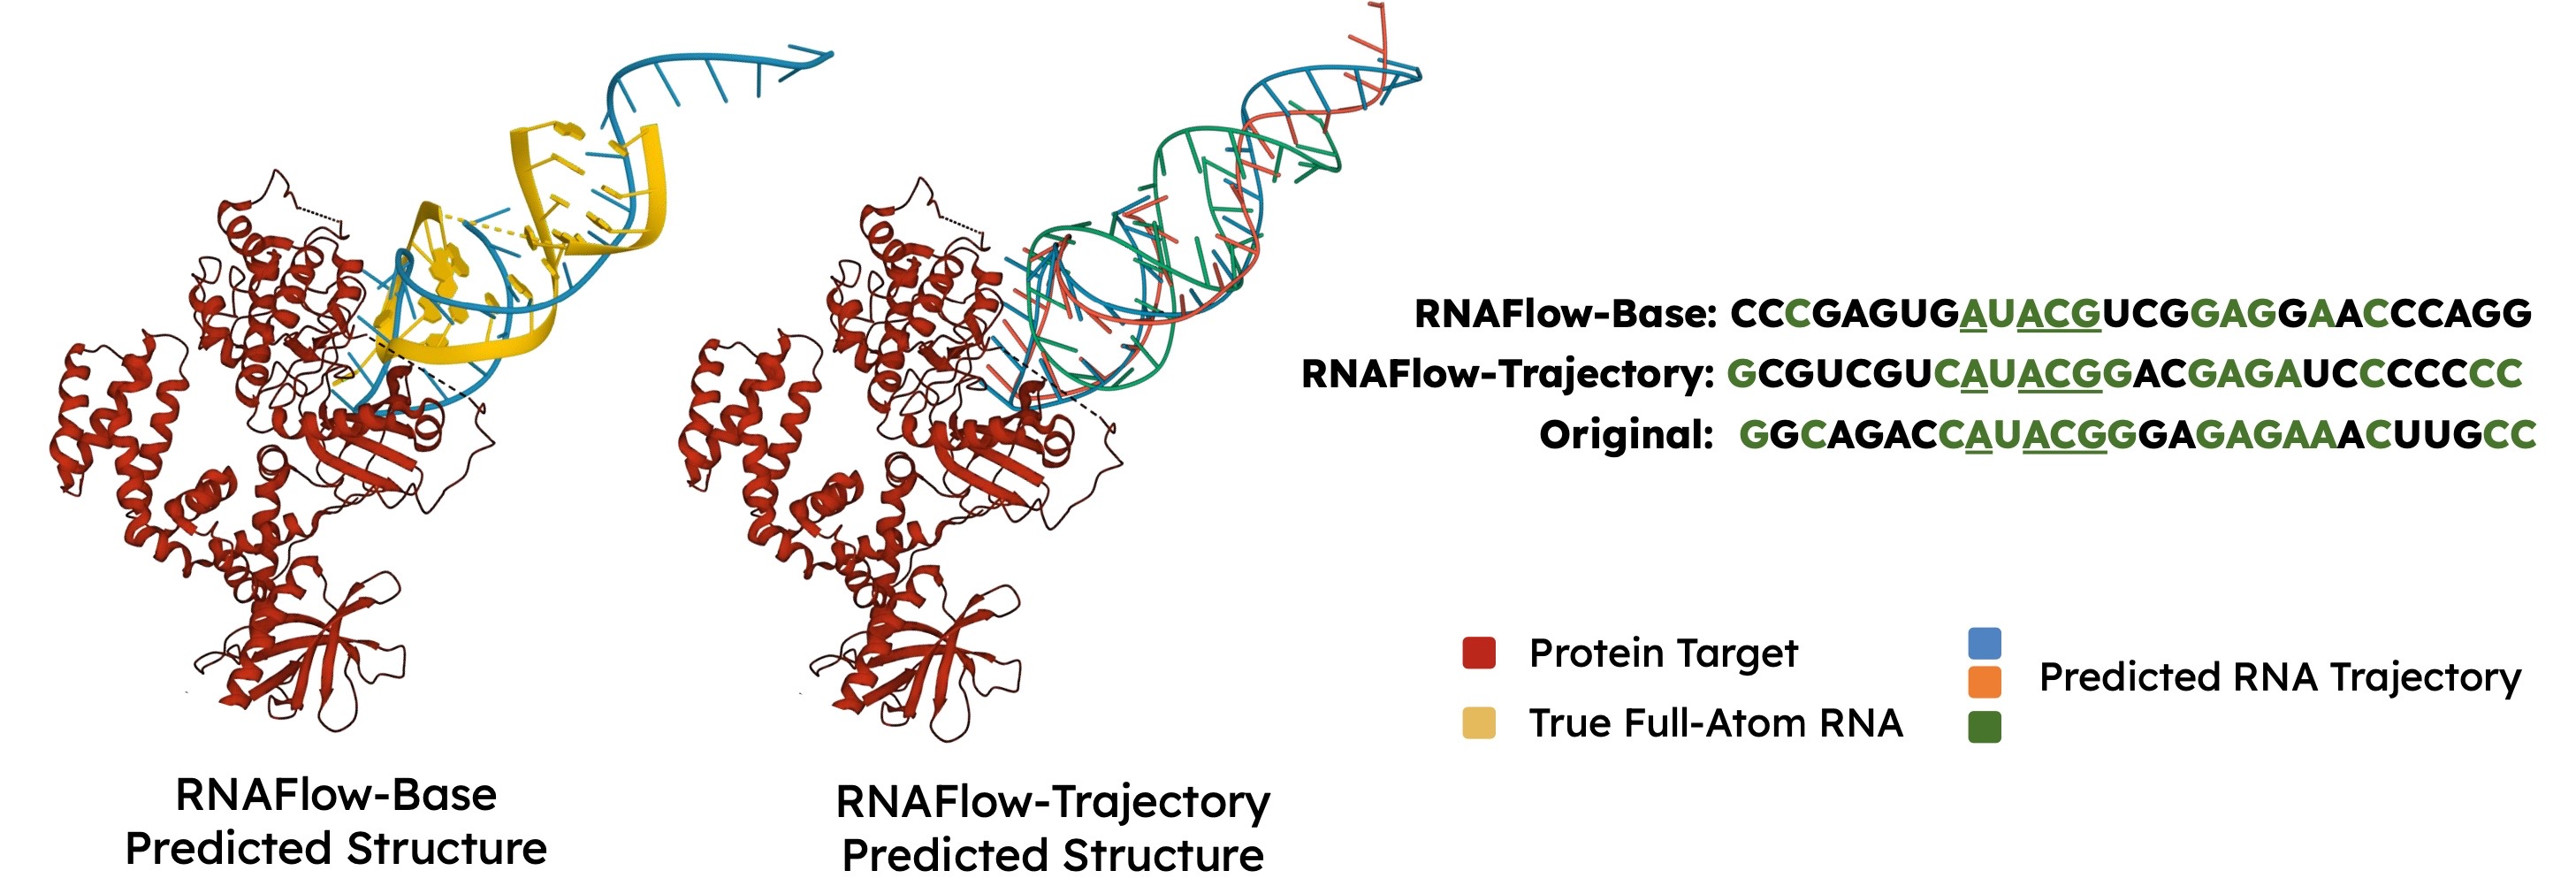
\includegraphics[width=2\columnwidth]{grk2.png}
    \caption{Structure and sequence RNAs designed by RNAFlow for GRK2 binding in motif-scaffolded setting. The predicted structure is Kabsch aligned onto the ground-truth for visualization. In the sequence designs, green-colored characters show nucleotides that are correctly recovered from the ground-truth. Underlined nucleotides are part of the given binding motif.}
    \label{fig:4}
\end{figure*}

On the sequence similarity split, the best RNAFlow model gives a $28\%$ improvement over random generation and a $33\%$ improvement over LSTM. Without rescoring, we see a $20\%$ improvement in recovery relative to the best baseline. We find that while the LSTM's performance degrades on the sequence similarity split, RNAFlow's performance is consistent. RNAFlow-Trajectory does not improve recovery, indicating that the generated trajectories may not approximate conformational ensembles as effectively when trying to generalize to biologically dissimilar RNAs. While the RNAFlow recovery rate does not reach the upper bound established by the inverse folding model, we note that for some proteins, our model designs new sequences that fold into the desired structure. For example, as shown Figure \hyperref[fig:3]{3a}, RNAFlow can design molecules that match the ground-truth structure with a relatively dissimilar sequence composition.


\subsection{Structure \& Sequence Novelty}
\label{sec:4.2}

We then evaluate the novelty of RNAs designed by RNAFlow-Base. Sequence novelty is quantified as $1 -$ sequence recovery of each generated sample to its most similar RNA sequence in the training set. Similarly, structure novelty is $1 - $ TM-score between a generated sample and its most similar RNA structure in the training set. We observe that the majority of sequence content in the generated RNAs is not observed in the training set, showing that RNAFlow can generalize and design novel RNAs. The generated structures are also reasonably novel.

\begin{table}[h]
    \centering
    \small
    \caption{Structure and sequence novelty of RNAs generated by RNAFlow-Base.}
    \vspace{0.05in}
    \renewcommand\thetable{3}
    \begin{tabular} {lcc@{\hskip 0.25in}cc}
        \hline
        & Sequence Novelty & Structure Novelty \\ \hline
        RF2NA Split & $0.55$ & $0.63$ \\
       Seq Sim Split & $0.63$ & $0.64$ \\
    \hline
    \end{tabular}
    \label{tab:3}
\end{table}

\subsection{Ablation Study}
\label{sec:4.3}

We conduct an ablation study to determine which components of our model contribute to its performance. As shown in Figure \hyperref[fig:3]{3b}, we report recovery rate and RMSD on the sequence similarity split under various conditions, since the sequence split is more general to a design setting. First, we fine-tune Noise-to-Seq on sequence cross-entropy only, removing the structure MSE loss. When this denoiser is used in the standard five-step inference loop, the RMSD increases by $1.25$ compared to RNAFlow-Base, and recovery rate decreases by $1$ percentage point. Next, we remove protein conditioning and find that RMSD increases by $2.52$, and recovery drops by $7$ percentage points, showing that providing protein information is important.

We assess the effect of our ``pose guess'' complex alignment method by performing inference with the true RNA centroid and protein orientation. While the recovery is not affected, the RMSD is $0.67$ better than our method. This shows that our initial pose prediction method does not degrade performance significantly. Finally, we show the performance when inference is performed with ten flow matching steps rather than five. While RMSD is better than our method by $0.25$, recovery is not affected. Given the insignificant impact on performance, we choose to use $5$ integration steps in favor of inference time speed-up.

\subsection{Motif-Scaffolded Design of RNAs for GRK2}
\label{sec:4.4}

\textbf{Design Procedure.} For this task, we train RNAFlow on all protein-RNA examples except the ground-truth GRK2-C28 protein-aptamer complex (PDB ID: 3UZS). Comparing against an LSTM and MMDiff, we evaluate the structure and sequence accuracy of GRK2-conditioned RNA design given a $4$-nucleotide binding site sequence motif. For all methods, we sample $10$ RNA designs and select $1$ top design by the output rescoring model. We report the recovery rate with respect to the true aptamer sequence of length $28$ and the RMSD with respect to its crystal structure. 

\textbf{Results.} As shown in Table \hyperref[tab:3]{3}, RNAFlow outperforms the baselines in terms of both RMSD and recovery. Compared to MMDiff, RNAFlow-Base gives an $8.16\%$ improvement in RMSD and $34.38\%$ improvement in recovery. As shown in Figure \hyperref[fig:4]{4}, the predicted structure resembles the ground-truth aptamer closer to the binding site, though the structure deviates when further away from the protein. 

\begin{table}[h]
    \centering
    \small
    \caption{GRK2 binder metrics.}
    \vspace{0.05in}
    \renewcommand\thetable{3}
    \begin{tabular} {lcc@{\hskip 0.25in}cc}
        \hline
        & RMSD & Recovery \\ \hline
        LSTM & - & $0.29$ \\
        MMDiff & $9.19$ & $0.32$ \\ \hline
        RNAFlow-Base & $8.44$ & $0.43$ \\
        RNAFlow-Trajectory & $\textbf{7.09}$ & $\textbf{0.54}$ \\ \hline
    \end{tabular}
    \label{tab:3}
\end{table}

Moreover, RNAFlow-Trajectory gives an $22.85\%$ improvement in RMSD and a $68.75\%$ improvement in recovery. Figure \hyperref[fig:4]{4} shows the predicted structural trajectory. One of the intermediate trajectory structures shown in green has a lower RMSD ($6.42$) than the final structure. However, inverse folding the intermediate structure alone yields a significantly lower recovery ($0.44$) than applying Traj-to-Seq ($0.54)$. Crucially, we observe that the sequence predicted by RNAFlow-Trajectory recovers nucleotides on either end of the aptamer, far away from the given binding motif. As noted by \citet{tesmer2012molecular}, these stem regions are critical for the aptamer's high affinity because they ``limit the number of possible conformations for the selected RNA.'' Thus, we argue that having conformational information is important to design these regions.

